\section{Multilayer mirror 1}
\subsection{Design}
The center of the first multilayer mirror of the BEATS DMM is positioned at 15.165 m from the ID photon source. \\
CINEL will verify the thermal stability of the ML1 with FEA simulations considering the white beam colliding with the mirror at the maximum Bragg angle allowed by the Bragg stage motorization (34.9 mrad). The thermal stability of the cooled mask in front of the ML1 profile shall be also verified.\\

\subsection{Input beam}
A beam snapshot at 15.165 m from source is shown in Figure \ref{fig:snapshot_ML1}.
\begin{figure}[ht]
\centering
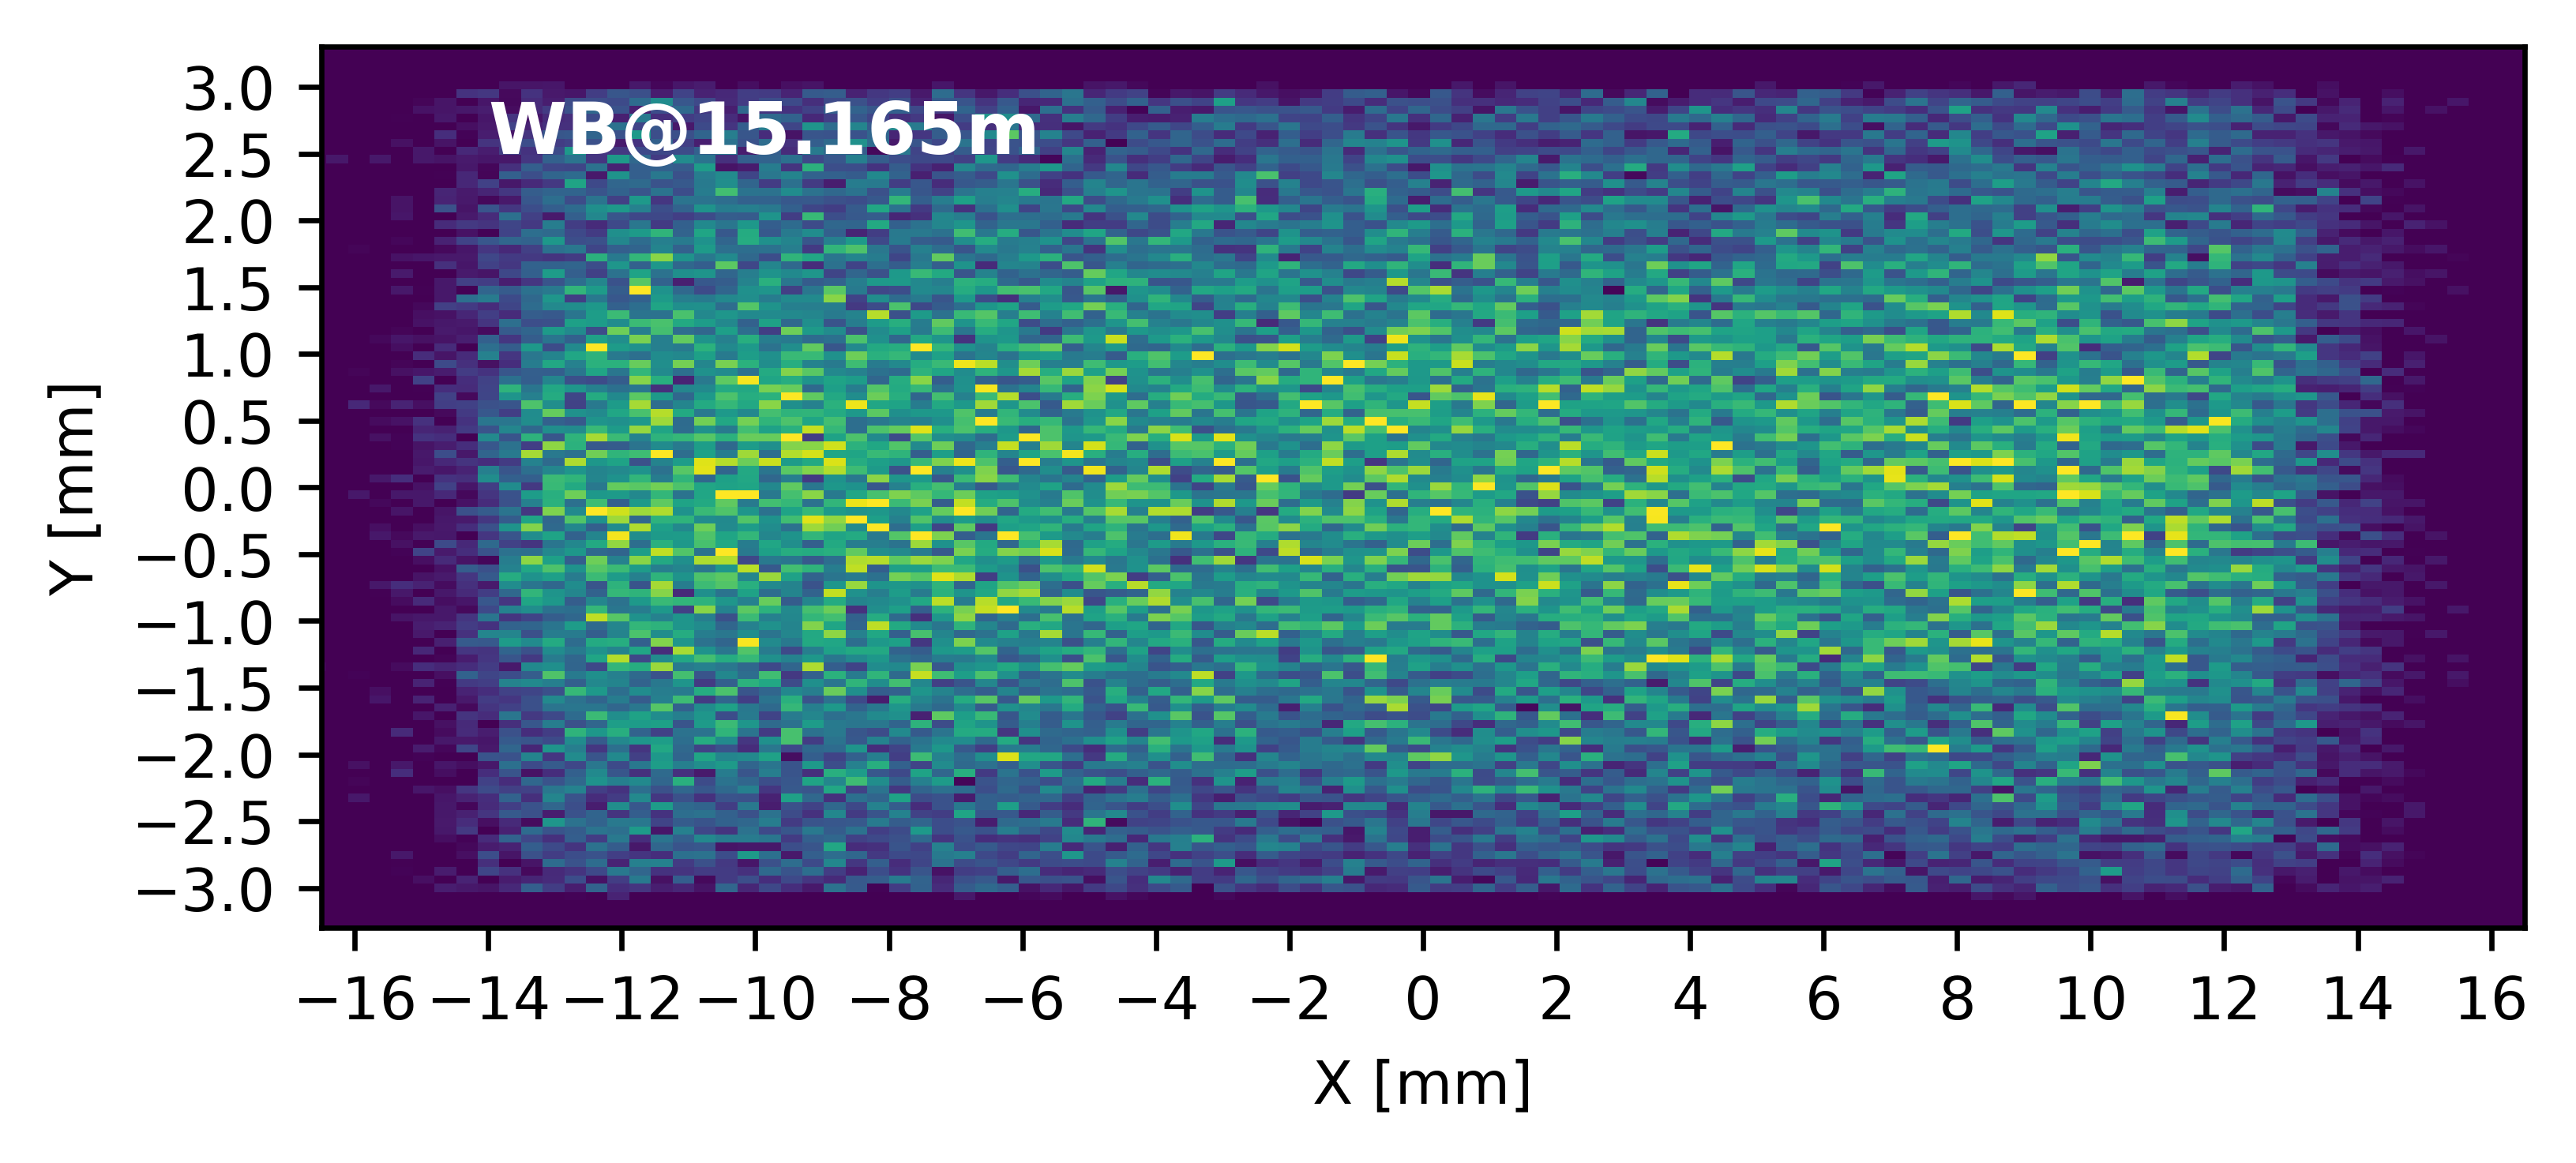
\includegraphics[width=0.8\textwidth]{images/WB_snapshot_15.165.png}
\caption{\label{fig:snapshot_ML1} White beam snapshot at 15.165 m from source (center position of ML1).}
\end{figure}

The power density profile at 15.165 m from source is shown in Figure \ref{fig:power_profile_ML1}. Raw data can be found in the \powerprofilesurl. \\
\begin{figure}[ht]
\centering
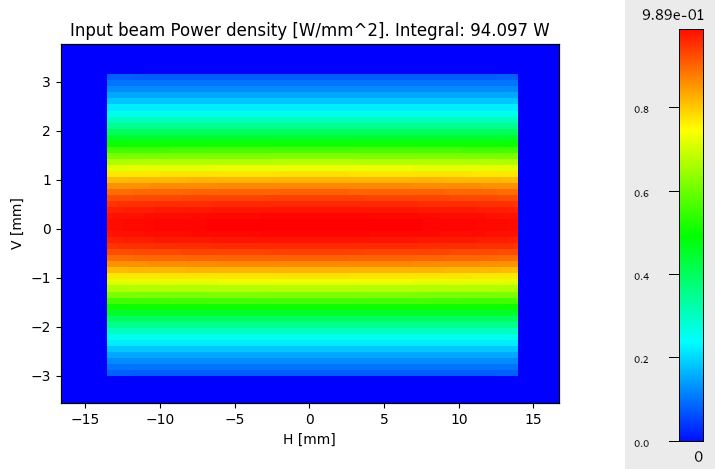
\includegraphics[width=0.8\textwidth]{images/power_profile_ML1.png}
\caption{\label{fig:power_profile_ML1} Power density profile at 15.165 m from source (center position of ML1).}
\end{figure}